
\section*{Problema P9.14}

\renewcommand*\thesection{9.14}
\numberwithin{equation}{section}

\begin{center}
    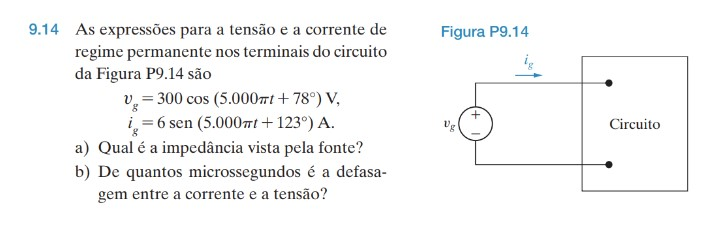
\includegraphics[scale=1.0]{P9.14.jpg}
\end{center}

\subsection*{(a)}

A impedância \(Z_{in}\) vista pela fonte é dada por

\begin{equation}\label{eq:9.14.1}
    Z_{in} = \frac{V_g}{I_g}
\end{equation}

Usando a relação trigonométrica 

\[  \sin{\theta} = \cos({\theta - 90^{\circ})}  \]

Podemos reescrever a expressão de \(i_g(t)\) como

\[ i_g(t) = 6\cos({5000\pi + 123^{\circ} - 90^{\circ}})  \]

\[ i_g(t) = 6\cos({5000\pi + 33^{\circ}})  \]

Assim, em notação fasorial, temos 

\begin{equation}\label{eq:9.14.2}
    Z_{in} = \frac{300\fase{78}}{6\fase{33}}
\end{equation}

\[ \boxed{Z_{in} = 50\fase{45} \; \Omega}  \]

\subsection*{(b)}

Usando proporcionalidade (regra de três simples), sabemos que uma 
diferença de fase de \(\Delta \phi \) corresponde a uma diferença 
temporal \(\Delta t \) dada por    


\[ \frac{T}{\Delta t} = \frac{360^{\circ}}{\Delta \phi}  \]

onde \(T = \frac{2\pi}{\omega} \) é o período do sinal. Isolando \(\Delta t \), temos

\begin{equation}\label{eq:9.14.3}
    \Delta t = T \frac{\Delta \phi}{360^{\circ}}
\end{equation}

\[  \Delta t = \frac{2\pi}{\omega} \frac{\Delta \phi}{360^{\circ}}  \]

Substituindo tudo, temos

\[ \boxed{\Delta t = 50 \; \mu s}  \]
